\section{Optimization}
Based on popup graphs, we only need three sets of key variables to define a popup craft design:
\begin{enumerate}
\item $a(f)$: A binary variable indicating the activeness of fold line $f$.
\item $c(f)$: A binary variable indicating the convexity of fold line $f$ (whether the fold line points outwards ($c(f) = 1$) or inwards ($c(f) = 0$).
\item $p(f)$: A integer variable indicating the position of fold line $f$.
\end{enumerate}

The goal is to determine these variables so that the popup graph satisfies four key properties: foldability, connectivity, stability and consistency. Additional properties can be enforced according to user input. We will explain each property and show how to formulate such property in our optimization framework.

\subsection{Foldability}
\textbf{Foldability Definition: }

\textbf{Variable Definition: }
We associate a set of variables $c(f)$ determining the convexity of $f$, that is . A set of variables $X(f)$ determining the X coordinate of $f$, and $Y(f)$ determining the Y coordinate of $f$.

There is $x(f) + y(f) = p_u(f)$ ($p(f) = (p_u(f), p_v(f))$).

The orientation constraints involve $c(f)$. For fold line neighbor pair $(f_l, f_r)$, there is:
\begin{equation}
  \begin{aligned}
    & c(f_l) = 1 - c(f_r) & \text{ if } a(f_r) = 1 \\
    & c(f_l) = c(f_r) & \text{ otherwise } \\
  \end{aligned}
\end{equation}

The position constraints is formed as:
\begin{equation}
  \begin{aligned}
    & x(f_l) < x(f_r) \quad & y(f_l) = y(f_r) & \text{ if } c(f_r) = 1 \\
    & x(f_l) = x(f_r) \quad & y(f_l) < y(f_r) & \text{ otherwise } \\
  \end{aligned}
\end{equation}

\subsection{connectivity}
Due to the fact that the number of segments is small in our image-based design process, we prefer one intriguing structure containing all segments instead of multiple separated simple structures.. For this reason, we enforce two type connectivity here. First, each patch should have at least one path from both left background patch and right background patch. Second, after taking background patches away, the rest graph should have only one connected component. The connectivity property is incorporated into the optimization formulation as follows.

As new fold lines will never be cut, the connectivity property is considered based on initial patches. The first type of connectivity is enforced by simply adding a constraint that each initial patch (except the background patch) has at least one active left initial fold line and one active right initial fold line. The proof is trivial as the graph has non-loop property. We re-phrase the second connectivity constraint as there exists at least one connection between any pair of patches (background patches are excluded). Here the connection exists when:

\begin{enumerate}
\item For a pair of neighboring patches, at least one fold line between them is active.
\item For a pair of non-neighboring patches, they both have connection with at least one other patch.
\end{enumerate}

Due to the symmetric definition of connection, we can simplify the constraint as there exists at least one connection between each patch and one denoted patch $s$. The denoted patch is a randomly picked non-background patch. Then we define the connection depth for each patch as the length of the shortest path to patch $s$. We use binary variable $c_{pd}$ to indicate whether patch $p$ has connection depth $d$ ($d \in [1, MAX\_DEPTH]$). Based on $c_{pd}$, the connectivity constraint is formulated as $\sum_d{c_{pd}} = 1$. According to the definition of connection, $c_{pd}$ subjects to:

\begin{equation*}
  \begin{cases}
    c_{p1} \leq \sum_{f \in F(p, s)}a(f) & \text{ If patch $p$ is a neighbor of $s$} \\
    c_{p1} = 0 & \text{ If patch $p$ is not a neighbor of $s$} \\
    c_{pd} <= \sum_{q \in N(p)}(c_{q(d-1)}\sum_{f \in F(p, q)}a(f))
  \end{cases}
\end{equation*}

Note that some patches do not have active fold lines because they lie inside another patch (see the eyes in the bear example). We call them ``island patches''. For island patches, connectivity no longer holds. For this reason, we add another set of binary variables $i(p)$ to indicate whether a patch is an island patch or not. We modify the above connectivity constraints so that they are disabled for island patches. And an island patch has no fold line, so there should be $a(f) <= 1 - i(p) \quad \forall f \in F(p)$.

\subsection{Stability}
We associate a set of binary variables $s(f)(d)$ indicating the stability of $f$ at depth $d$. Here the depth can be interpolated as the following procedure. $Lf$, $Rf$, and all fold lines on the background patches are stable at depth 0. Now if we add two patches between background patches forming a stable structure, the corresponding fold line will be stable at depth 1. We can continue to add stable structure based on current structure and the depth increases as the procedure goes on.

We use the idea of forming the popup by iteratively adding stable structure to formulate the stability constraint. That is, we check a building block at depth $d$ to see whether it is stable or not based on previous building blocks (with stability depth less than $d$).


% Note that we only consider stability for active fold lines. A key additional variable $same\_patch(f_s, f_t)$ indicates whether $f_s$ and $f_t$ are on the same final patch. $same\_patch(f_s, f_t) = 1$ when $P(f_s, f_t)$ exists and its fold lines are all inactive (meaning the patch is not folded). (See figure \ref{fig:path}.) With $same\_patch(f_s, f_t)$, we can sum up with support from all fold lines on the same patch to form constraints as $\#(f_t) <= \sum_s{*(f_s)c(f_s, f_t)}$ (see figure \ref{fig:support} for details).

% \begin{figure}[h]
%   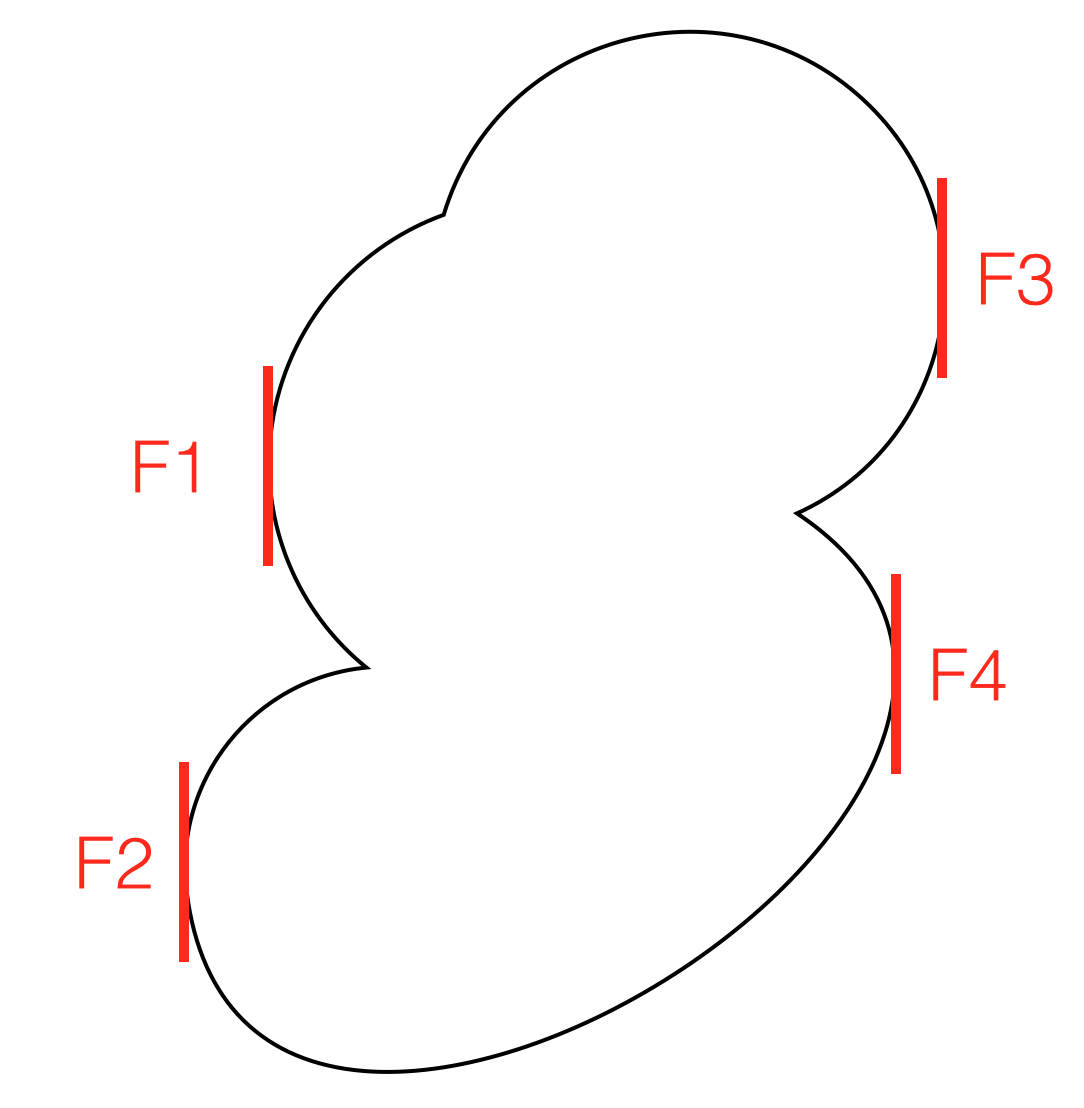
\includegraphics[width = 0.3\textwidth]{Figures/support}
%   \caption{Suppose these four fold lines are on the same final patch (determined by same\_patch($f_i$, $f_j$) = 1). Then the attribute for each fold line results from the support from all these four fold lines. To be more specific, for these four fold lines, we have the following. 1) If two or more fold lines are stable, then other fold lines are also stable. 2) If one fold line is stable, then other fold lines is called as ``directly connected'' which means a fold line is directly connected with a stable fold line (has only one degree of freedom). 3) If two or more fold lines are ``directly connected'', then other fold lines are called ``double-connected'' which means a fold line is not directly connected with stable fold lines but has two connection with stable fold lines. 4) If one fold line is ``double-connected'', then other fold lines is called as ``extended'' (used for certain cases).}
%   \label{fig:support}
% \end{figure}

% With the notation in figure \ref{fig:support}, a fold line is stable if one of the follows holds:

% \begin{enumerate}
% \item It is on the same patch with two stable fold lines.
% \item It is ``directly connected'' with a stable patch from the left and ``directly connected'' with a stable patch from the right.
% \item It is ``double-connected'' with a stable patch from the left and ``double-connected'' with a stable patch from the right.
% \item It is ``directly connected'' with a stable patch from the left and ``double-connected'' with a stable patch from the right (or vice versa).
% \item It is ``extended'' with a stable patch from the left and ``double-connected'' with a stable patch from the right (or vice versa).
% \end{enumerate}

We consider five types of stable structure:
\begin{enumerate}
\item A fold line is stable if it is on the same patch with two known stable fold lines. (\cite{li2010popup})
\item A fold line is stable if it is on the same patch with one known stable fold line and on another patch with another known stable fold line. (\cite{li2010popup})
\item A fold line is on a B-path or F-path. (\cite{le2014surface})
\item A fold line is double connected with two stable patches (ours).
\item A fold line is double connected with a stable patch and directly connect with a stable patch (or a patch which is double connected with a stable patch) (ours).
\end{enumerate}

    These cases are illustrated in figure \ref{fig:stable}.

\begin{figure}[h]
  
\includegraphics[width = 0.2\textwidth]{Figures/stable_1}
  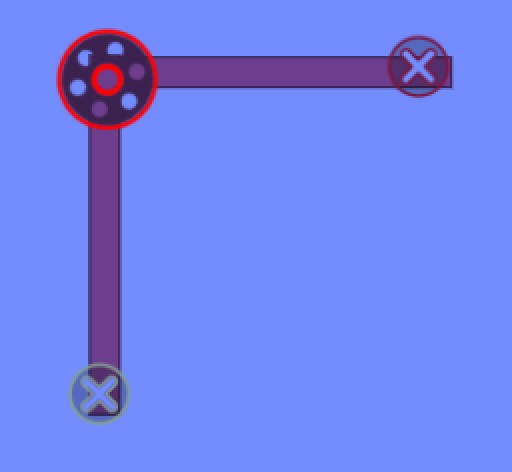
\includegraphics[width = 0.2\textwidth]{Figures/stable_2}
  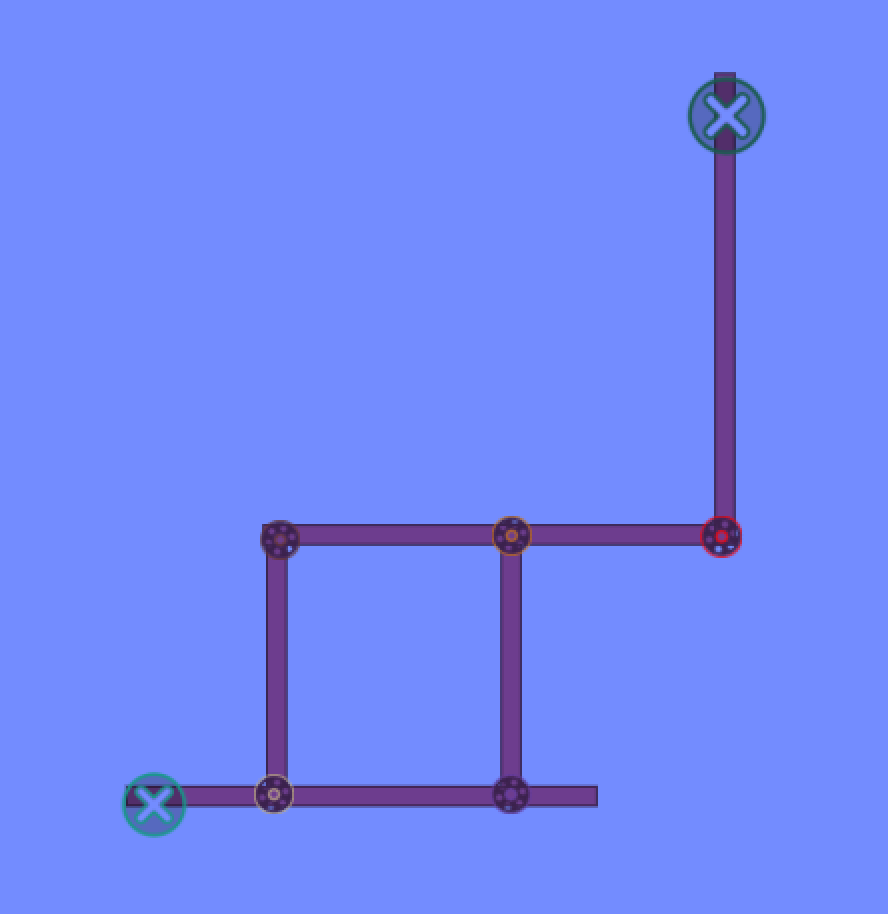
\includegraphics[width = 0.2\textwidth]{Figures/stable_3}
  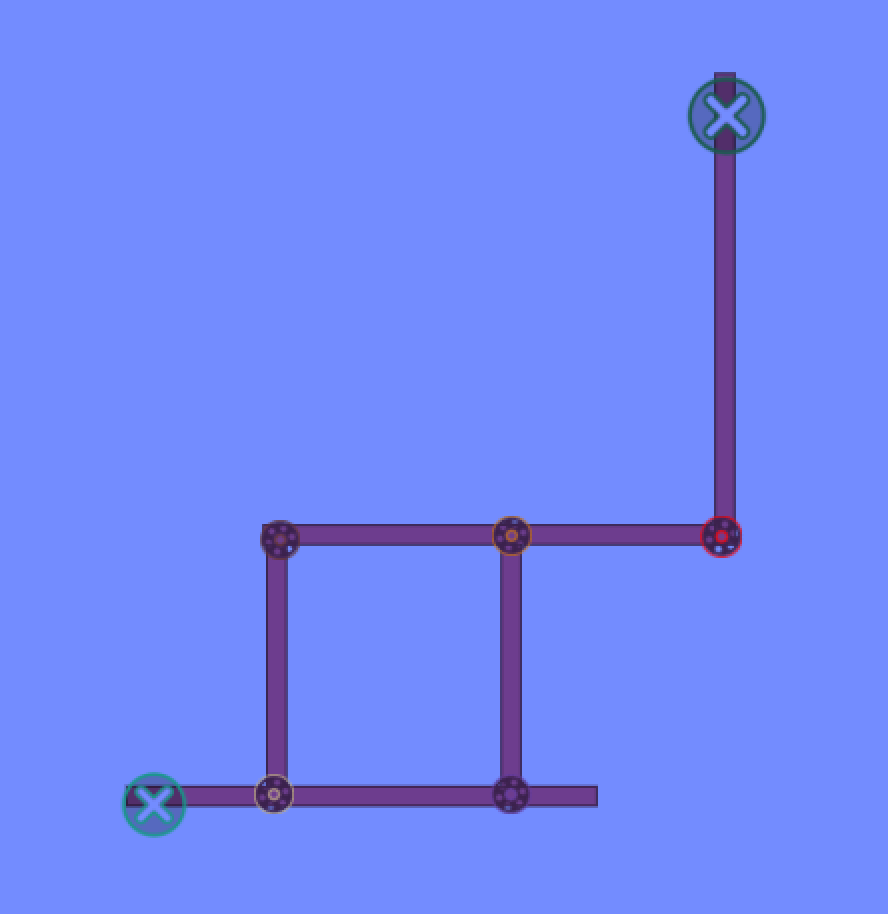
\includegraphics[width = 0.2\textwidth]{Figures/stable_4}
  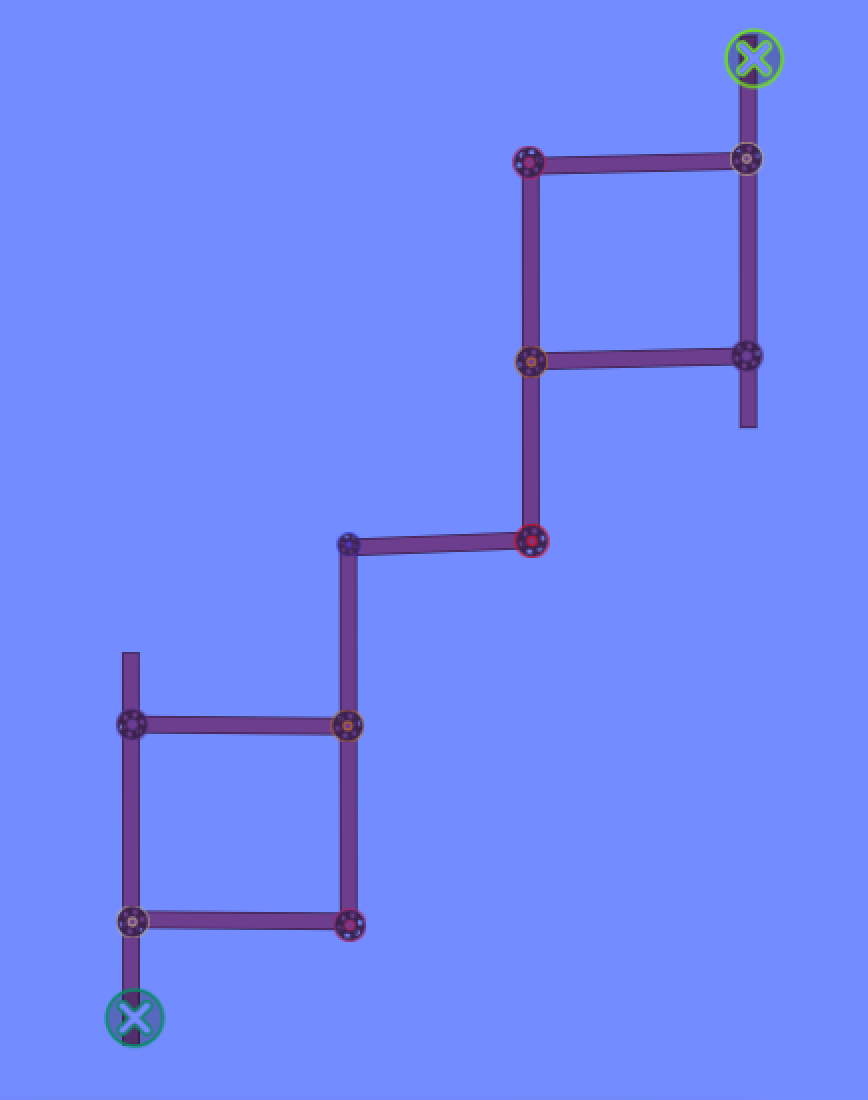
\includegraphics[width = 0.2\textwidth]{Figures/stable_5}
  \caption{The anchor with X sign represents a stable fold line and the anchor with red color is the fold line to be considered}
  \label{fig:stable}
\end{figure}

The process of determining stability is as follows:
\begin{enumerate}
\item Background fold lines are stable with stability depth 0.
\item For stability depth k, we find either the above structures based on the stable fold lines with stability depth less than k, and mark fold line in such structures as stable with stability k.
\item Repeat this process until all fold lines are marked as stable at some point. (We set a stability depth limit in practice.)
\end{enumerate}
\subsection{Consistency}
As we design the popup craft based on the input image, we want the design result to follow the input shape. Some geometry changes are avoidable since we need to add fold lines between patches, but still we want to minimize the geometry change. Although more complicated metric could be applied here, we use a simple metric to measure the geometry change. That is, the geometry change for a fold line is the amount of shift from its initial location to its final location, and the geometry change for the design result is the summation of fold line geometry changes. So the consistency is measured as: -$\lambda_{pos}\sum_f(pos(f) - pos_i(f))^2$.